%----------------------------------------------------------------------------------------
%	PACKAGES AND OTHER DOCUMENT CONFIGURATIONS
%----------------------------------------------------------------------------------------

\documentclass[twoside]{article}

\usepackage[sc]{mathpazo} % Use the Palatino font
\usepackage[T1]{fontenc} % Use 8-bit encoding that has 256 glyphs
\linespread{1.05} % Line spacing - Palatino needs more space between lines
\usepackage{microtype} % Slightly tweak font spacing for aesthetics

\usepackage[english]{babel} % Language hyphenation and typographical rules

\usepackage[hmarginratio=1:1,top=32mm,columnsep=20pt]{geometry} % Document margins
\usepackage[hang, small,labelfont=bf,up,textfont=it,up]{caption} % Custom captions under/above floats in tables or figures
\usepackage{booktabs} % Horizontal rules in tables

\usepackage{lettrine} % The lettrine is the first enlarged letter at the beginning of the text

\usepackage{enumitem} % Customized lists
\setlist[itemize]{noitemsep} % Make itemize lists more compact

\usepackage{titlesec} % Allows customization of titles
\renewcommand\thesection{\Roman{section}} % Roman numerals for the sections
\renewcommand\thesubsection{\roman{subsection}} % roman numerals for subsections
\titleformat{\section}[block]{\large\scshape\centering}{\thesection.}{1em}{} % Change the look of the section titles
\titleformat{\subsection}[block]{\large}{\thesubsection.}{1em}{} % Change the look of the section titles

\usepackage{fancyhdr} % Headers and footers
\pagestyle{fancy} % All pages have headers and footers
\fancyhead{} % Blank out the default header
\fancyfoot{} % Blank out the default footer
\fancyhead[C]{Third Order Tensors with Application $\bullet$ May 2018} % Custom header text
\fancyfoot[RO,LE]{\thepage} % Custom footer text

\usepackage{titling} % Customizing the title section

\usepackage{hyperref} % For hyperlinks in the PDF

\usepackage{multicol}
\usepackage{graphicx}
\graphicspath{{img/}}
\usepackage{float}

\usepackage{amssymb,amsmath,amsthm}
\newtheorem{theorem}{Theorem}
\newtheorem{defn}{Definition}

\newcommand{\code}[1]{\texttt{#1}}

%----------------------------------------------------------------------------------------
%	TITLE SECTION
%----------------------------------------------------------------------------------------

\setlength{\droptitle}{-4\baselineskip} % Move the title up

\pretitle{\begin{center}\Huge\bfseries} % Article title formatting
\posttitle{\end{center}} % Article title closing formatting
\title{Third Order Tensors with Application} % Article title

\author{%
\textsc{Ivan \v{C}eh}\\% \\[1ex] 
\normalsize Computer Science \\
\normalsize \href{mailto:ivan.ceh1234@gmail.com}{ivan.ceh1234@gmail.com} 
\and
\textsc{Petra Br\v{c}i\'c}\\% \\[1ex] 
\normalsize Applied Mathematics \\
\normalsize \href{mailto:petrabrcic94@gmail.com}{petrabrcic94@gmail.com} 
\and
\textsc{Sandro Lovni\v{c}ki}\\% \\[1ex] 
\normalsize Computer Science \\ 
\normalsize \href{mailto:lovnicki.sandro@gmail.com}{lovnicki.sandro@gmail.com}
}

\date{\today} 
\renewcommand{\maketitlehookd}{%
\noindent \textbf{\\Abstract:} Operations with tensors, or multiway arrays, have become increasingly prevalent in recent years. In this paper, we explore a theoretical framework for manipulating  such objects and derive basic operators on them, keeping the structure closed and also robust, in a sense that operators on lower dimensions can be generalized in this higher order framework. Also, we present application of third-order tensors on two examples; image deblurring and face recognition.
\\\\
\textbf{Keywords:} third order tensor, t-product, t-SVD, t-CG, deblurring, face recognition.
}


%----------------------------------------------------------------------------------------

\begin{document}

% Print the title and table of contents
\maketitle
\tableofcontents
\newpage

%----------------------------------------------------------------------------------------
%	ARTICLE CONTENTS
%----------------------------------------------------------------------------------------
\begin{multicols}{2}

\section{Introduction}
A tensor is a multi-dimensional array of numbers. For example, we could say that vector $v \in \mathbb{R}^{n_1}$ is a first-order tensor and similarily, matrix $M \in \mathbb{R}^{n_1 \times n_2}$ is a second-order tensor. Therefore, a third-order tensor is $\mathcal{A} \in \mathbb{R}^{n_1 \times n_2 \times n_3}$.\\
\indent In this paper, we provide a setting in which the familiar tools of linear algebra can be extended to better understand third-order tensors. Significant contributions to extending matrix analysis has been made in the works of Misha E. Kilmer and others in \cite{kilmer-braman-hao} and \cite{kilmer-martin}.\\
\indent In sections that follow, we first introduce the basic notions and definitions of this new framework. We present methods which will be used in applictions and continue with two examples (image deblurring and face recognition), for which our Octave code can be found at our \hyperref[https://github.com/Qkvad/3rdOrderTensors]{GitHub repository}\footnote{https://github.com/Qkvad/3rdOrderTensors}.

\section{Theoretical Framework}
In this section, we will first describe notation that is convenient for manipulating third-order tensors and which will be used throughout the paper. Also, we define basic operations on tensors (multiplication, inverse, transpose) which lead us to tensors factorization algorithms and solvers; t-SVD and t-CG.

\subsection{Notation and Conversions}
Each third-order tensor $\mathcal{A} \in \mathbb{R}^{l \times m \times n}$ can be viewed as $n$ $l \times m$ matrices stacked upon eachother. Furthermore, it can also be viewed as a $l \times m$ matrix of vectors of length $n$. It is convenient to break tensor into "slices" and "tubal elements".
\begin{defn} Let $\mathcal{A} \in \mathbb{R}^{l \times m \times n}$. We introduce the following notation:
\begin{itemize}
	\item $i$-th \textbf{frontal slice} $\mathcal{A}^{(i)} \equiv \mathcal{A}(:,:,i)$
	\item $i$-th \textbf{lateral slice} $\overrightarrow{\mathcal{A}}_i \equiv \mathcal{A}(:,i,:)$
	\item $i,k$-th \textbf{tubal scalar} $\textbf{a}_{ik} \equiv \mathcal{A}(i,k,:)$
\end{itemize}
\end{defn}

In order to define tensor multiplication, we now present some conversions between tensor and matrix objects. To wrap a tensor into a matrix, functions \code{circ} and \code{matvec} will be used, and to unwrap a tensor from the return value of \code{matvec}, we use \code{foldn} operator. How those operators work on tensors and matrices is now presented.
\[
\code{circ}(\mathcal{A}) =
  \begin{bmatrix}
    \mathcal{A}^{(1)} & \mathcal{A}^{(n)} & \dots & \mathcal{A}^{(2)} \\
    \mathcal{A}^{(2)} & \mathcal{A}^{(1)} &  \dots  & \mathcal{A}^{(3)} \\
    \vdots            & \vdots            &  \ddots & \vdots \\
    \mathcal{A}^{(n)} & \mathcal{A}^{(n-1)} &  \dots & \mathcal{A}^{(1)} 
  \end{bmatrix}
\]

\[
\code{matvec}(\mathcal{A}) =
  \begin{bmatrix}
    \mathcal{A}^{(1)} \\
    \mathcal{A}^{(2)} \\
    \vdots            \\
    \mathcal{A}^{(n)} 
  \end{bmatrix}
\]

\noindent Correspondingly, \code{foldn} operator is defined so that \code{foldn}(\code{matvec}($\mathcal{A}),n$) = $\mathcal{A}$.

\subsection{Tensor Operators}
Now, with established notation and conversions, we are equipped to define needed tensor operators.

\begin{defn} Let $\mathcal{A} \in \mathbb{R}^{l \times p \times n}$ and $\mathcal{B} \in \mathbb{R}^{p \times m \times n}$. The t-product\footnote{our Octave implementation of t-product is called \code{tproduct}.} $\mathcal{A} \ast \mathcal{B}$ is a $l \times m \times n$ tensor defined as
\[ \mathcal{A} \ast \mathcal{B} := \code{foldn}(\code{circ}(\mathcal{A}) \cdot \code{matvec}(\mathcal{B}) ,n) \]
\end{defn}

There is also another algorithm for computing $\mathcal{A} \ast \mathcal{B}$ which uses fast Fourier transform (FFT). We compute $\hat{\mathcal{A}} = \code{fft}(\mathcal{A},[],3)$ which is a tensor obtained by applying FFT along each tubal scalar of $\mathcal{A}$. The same procedure is done for $\mathcal{B}$, then with the product of each pair of frontal slices of $\hat{\mathcal{A}}$ and $\hat{\mathcal{B}}$ we get frontal slices of $\hat{\mathcal{C}}$ and then the desired product $\mathcal{C} := \mathcal{A} \ast \mathcal{B}$ is obtained by applying the inverse FFT on $\hat{\mathcal{C}}$, i.e. $\mathcal{C} = \code{ifft}(\hat{\mathcal{C}},[],3)$.

Similarly, the inverse of tensor $\mathcal{A}$ is computed by applying FFT on $\mathcal{A}$, inverting each frontal slice and then applying \code{ifft} on resulting tensor to obtain $\mathcal{A}^{-1}$.

\begin{defn} The $m \times m \times n$ identity tensor $\mathcal{I}_{mmn}$ is the tensor whose first frontal slice is an $m \times m$ identity matrix and all other frontal slices are all zeros. 
\end{defn}

\begin{defn} If $\mathcal{A} \in \mathbb{R}^{l \times m \times n}$, then $\mathcal{A}^T \in \mathbb{R}^{m \times l \times n}$ is obtained by transposing each frontal slice and reversing the order of frontal slices $2$ to $n$.
\end{defn}

It could be observed that $m \times 1 \times n$ tensors are just matrices oriented laterally. Furthermore, we could twist a $m \times n$ matrix to make a $m \times 1 \times n$ tensor. Following this line of thought, we introduce operators \code{twist} and \code{squeeze} defined as
\[ \code{squeeze}(\overrightarrow{\mathcal{A}}) = A \in \mathbb{R}^{m \times n} \]
\[ \code{twist}(\code{squeeze}(\overrightarrow{\mathcal{A}})) := \overrightarrow{\mathcal{A}} \]

\noindent Observing the established setting, it is useful to introduce $\mathbb{K}^m_n$ - the set of all $m \times n$ matrices oriented as $m \times 1 \times n$ tensors. For convenience, we write just $\mathbb{K}_n$ when $m=1$ and use it to represent the set of all tubal scalars of length $n$. As we mentioned before, $l \times m \times n$ tensor can be viewed as a $l \times m$ matrix of tubal scalars, so it is natural to say that $K^{l \times m}_n$ is the set of all $l \times m \times n$ tensors, i.e. $K^{l \times m}_n \equiv \mathbb{R}^{l \times m \times n}$.

This new definitions have as a consequence the consistency of operations on $\mathbb{K}^{l \times m}_n$ which we stress in the following list:
\begin{enumerate}
	\item multiplication, factorization, etc. based on t-product reduce to the standard matrix operations and factorizations when $n=1$.
	\item outer-products of matrices are well-defined.
	\item given $\overrightarrow{\mathcal{X}}, \overrightarrow{\mathcal{Y}} \in \mathbb{K}^m_n$, $\overrightarrow{\mathcal{X}}^T \ast \overrightarrow{\mathcal{Y}}$ is a scalar.
\end{enumerate}

\subsection{Factorizations}
Third order tensors can be viewed as operators. Specifically, for $\mathcal{A} \in \mathbb{R}^{l \times m \times n}$ and $\mathcal{X} \in \mathbb{R}^{m \times p \times n}$, the product $\mathcal{A} \ast \mathcal{X}$ defines a linear map from space of $m \times p \times n$ tensors to the space of $l \times p \times n$ tensors.

It is natural to observe tensors as operators on "twisted matrices", e.g. $m \times 1 \times n$ tensors, where \code{tproduct} defines a linear operator from $m \times n$ to $l \times n$ matrices.

\begin{defn} t-SVD, t-CG, t-QR,... all exist.
\end{defn}

%------------------------------------------------

\section{Image Deblurring}
In this section, we present the application of previously established theoretical framework around third-order tensors to the problem of image deblurring.\\

Generally, image deblurring problem is set as follows: Find the matrix $X$ representing the original image, having available the matrix $B = A X$, where $A$ is some blurring operator.\\

The problem is easily translated into the world of tensors and we have to find a twisted matrix $\overrightarrow{\mathcal{X}} \in R^{l \times 1 \times n}$, having $\overrightarrow{\mathcal{B}}$ and tensor operator $\mathcal{A}$ such that $\mathcal{A} \ast \overrightarrow{\mathcal{X}} = \overrightarrow{\mathcal{B}}$.\\

For the purposes of our demonstration, we will use rectangular images of size $m \times m$. First we need to create a tensor blurring operator $\mathcal{A} \in \mathbb{R}^{m \times m \times n}$. As suggested in \cite{kilmer-braman-hao} and \cite{kilmer-martin}, those blurring operators should have a specific structure of \textit{block Toeplitz} matrices with values obtained by \textit{Gaussian point spread function} (PSF).\\

We obtain out blurred tensor $\overrightarrow{\mathcal{B}}$ by applying the descibed blurring operator $\mathcal{A}$ on twisted original image $\overrightarrow{\mathcal{X}}$.
To find an approximation of original image, we use our \code{tCG} algorithm implemented in Octave whose detailed description is given below.\\

\noindent $[\overrightarrow{\mathcal{R}}_0,a] = \code{Normalize}(\overrightarrow{\mathcal{B}})$\\
$\overrightarrow{\mathcal{P}}_0 = \overrightarrow{\mathcal{R}}_0$\\
$\code{for}\ i=1:...$\\
\indent $c = (\overrightarrow{\mathcal{P}}^T \ast \mathcal{A} \ast \overrightarrow{\mathcal{P}})^{-1} \ast (\overrightarrow{\mathcal{R}}^T \ast \overrightarrow{\mathcal{R}})$\\
\indent $\overrightarrow{\mathcal{X}}_i = \overrightarrow{\mathcal{X}}_{i-1} + \overrightarrow{\mathcal{P}}_{i-1} \ast c$\\
\indent $\overrightarrow{\mathcal{R}}_i = \overrightarrow{\mathcal{R}}_{i-1} - \mathcal{A} \ast (\overrightarrow{\mathcal{P}}_i \ast c)$\\
\indent $d = (\overrightarrow{\mathcal{R}}^T_{i-1} \ast \overrightarrow{\mathcal{R}}_{i-1})^{-1} \ast (\overrightarrow{\mathcal{R}}^T_i \ast \overrightarrow{\mathcal{R}}_i)$\\
\indent $\overrightarrow{\mathcal{P}}_i = \overrightarrow{\mathcal{R}}_i + \overrightarrow{\mathcal{P}}_{i-1} \ast d$\\
\code{end}\\
$\overrightarrow{\mathcal{X}} = \overrightarrow{\mathcal{X}} \ast a$.\\

\noindent Our results can be seen in Figure \ref{fig:resdeblur}\\

\begin{figure}[H]
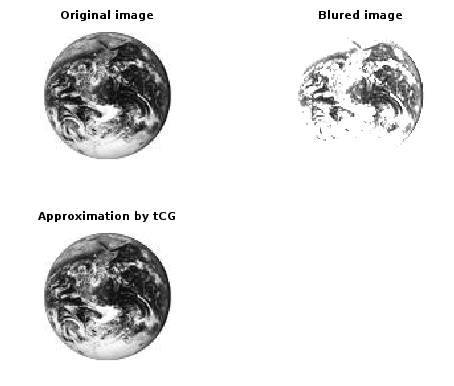
\includegraphics[width=0.5\textwidth]{res}
\caption{Results with $\sigma=2$. Numeber of iterations for tCG is 6.}
\label{fig:resdeblur}
\end{figure}

\section{Face Recognition}
We used AT\&T training set which consists of $400$ gray-scale images of size $112 \times 92$: $10$ photos of $40$ different persons. We divided them to training set with $7$ images of each person and test set with $3$ images of each person. For each person we create a tensor of size $112 \times 7 \times 92$ where images are placed as lateral slices.

We used the truncated t-SVD with first $k$ slices of tensor $U$ and used it to calculate the distance between each image $A_j$ in the test set and its orthogonal projection $U_k U_k^T A_j$. We suppose each image in test set should have the lowest distance between its ortogonal projection created by tensor of images of the same person. We tested this for different values of $k$.\\

\begin {tabular}{|r|l|}
\hline
k & accuracy \\
\hline
2 & 25\% \\
3 & 35\% \\
4 & 46.67\% \\
5 & 55.83\% \\
6 & 77.5\% \\
\hline
\end {tabular}

%------------------------------------------------


%----------------------------------------------------------------------------------------
%	REFERENCE LIST
%----------------------------------------------------------------------------------------

\begin{thebibliography}{99}

\bibitem[1]{kilmer-braman-hao}
Misha E. Kilmer, Karen Braman, Ning Hao.
\newblock Third Order Tensors as Operators on Matrices: A
Theoretical and Computational Framework with
Applications in Imaging

\bibitem[2]{kilmer-martin}
Misha E. Kilmer, Carla D. Martin.
\newblock Factorization Strategies for Third-order Tensors

 
\end{thebibliography}

%----------------------------------------------------------------------------------------

\end{multicols}{2}
\end{document}
